\subsection{Loss Tangent, ESR and Quality} \label{subsec:LossTangent}

Real components are not purely reactive and will have resistance in them, so their impedance vector will not be pointing straight up or down the imaginary axis as shown on figure \refq{fig:4_1_1_LossTangent1} and in section \refq{sec:ImpedanceAnalysis}.

\begin{figure}[H]
    \centering
    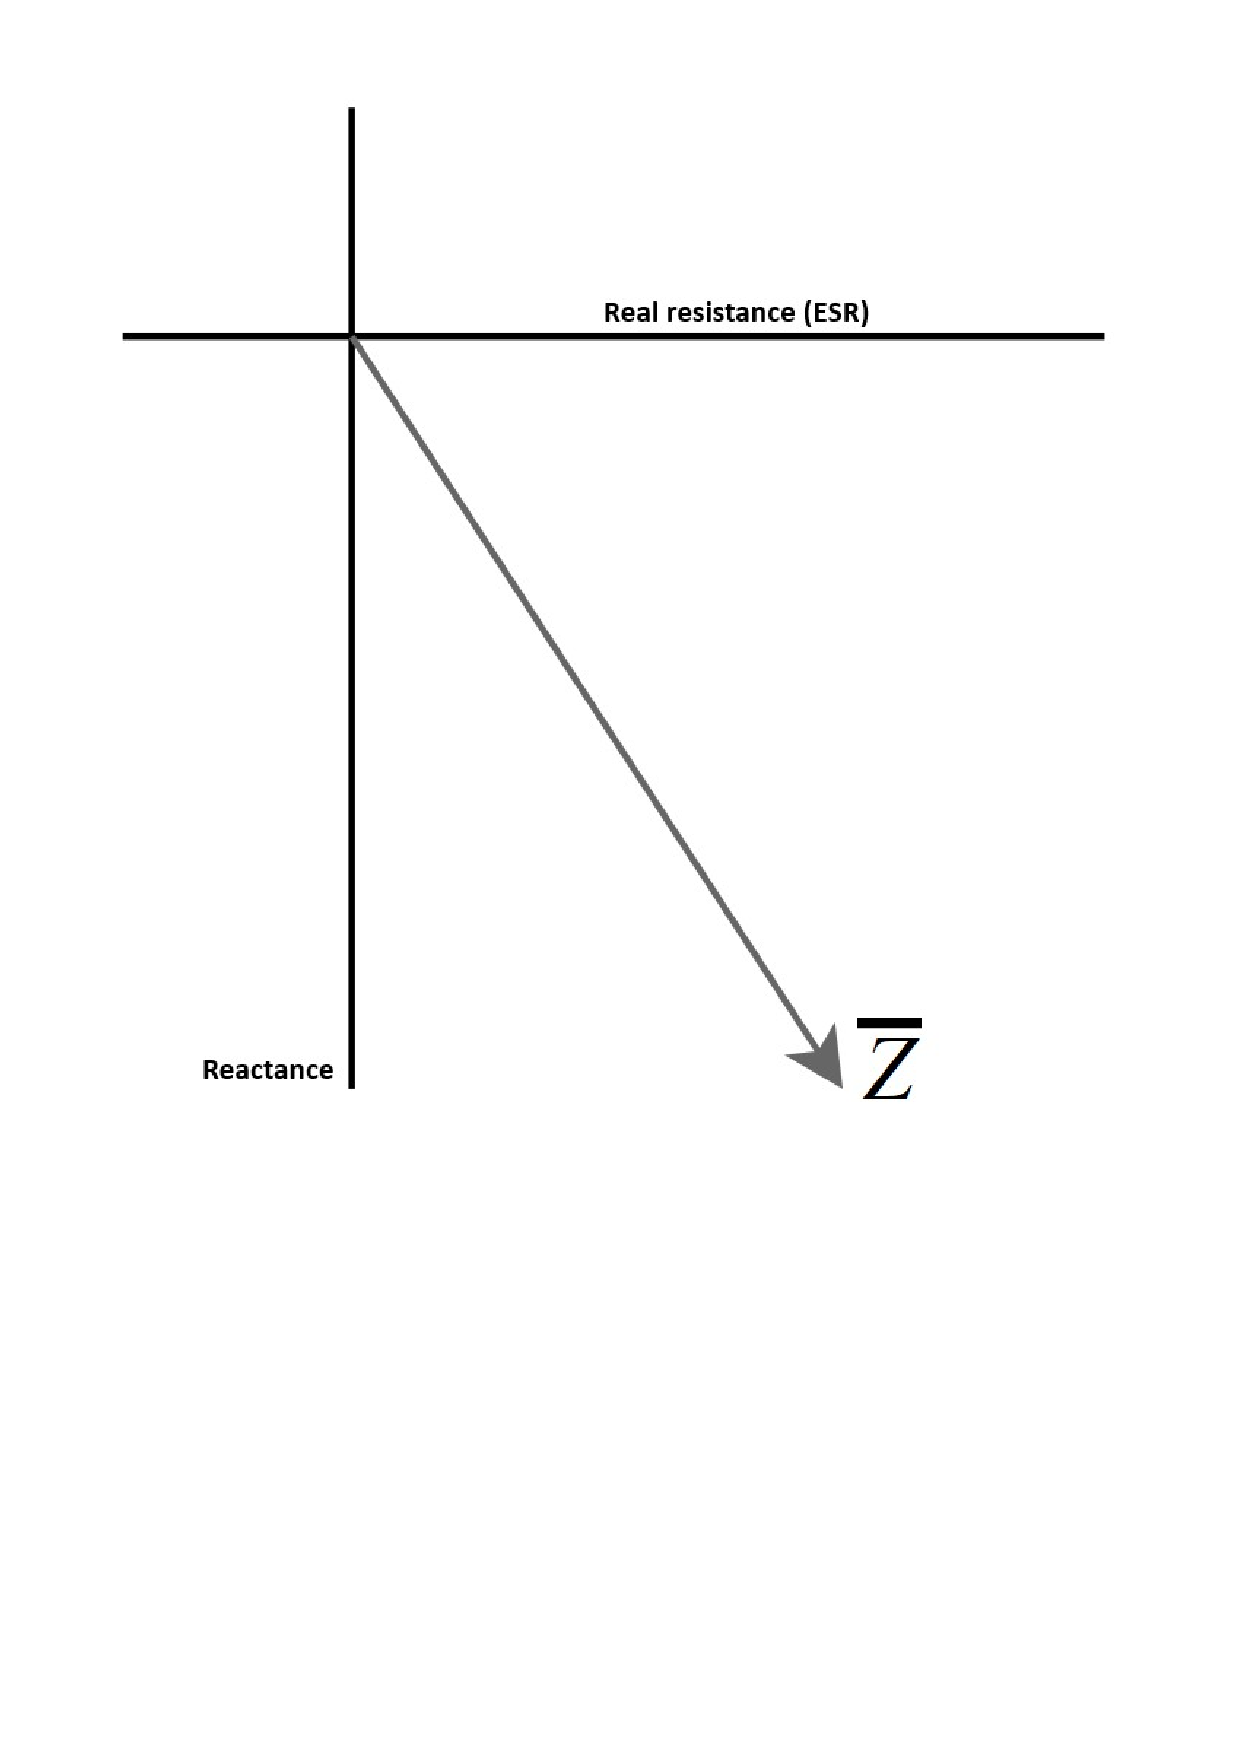
\includegraphics[clip, trim=0 250 0 0, width=0.4\textwidth]{Sections/4_TechnicalAnalysis/Figures/4_1_4_LossTangent1.pdf}
    \caption{The capacitor is not ideal. It has a finite amount of resistance in the materials it is made of.}
    \label{fig:4_1_1_LossTangent1}
\end{figure}

The impedance $|\bar Z|$ is a vector sum of the components real resistance (ESR) and the components reactance. A \textit{large} ESR (equivalent series resistance) will cause the impedance to deviate from the ideal pure reactance of the component and the losses in the device will increase as power can be dissipated in real resistances.

The angle between the impedance and the ideal reactance axis is called the \textit{loss angle} and is sometimes stated in component datasheets. It relates the resistance of a device to it's reactance. A large angle means the capacitor has large resistance and vice versa. This angle is shown on figure and is denoted $\delta$.

\begin{figure}[H]
    \centering
    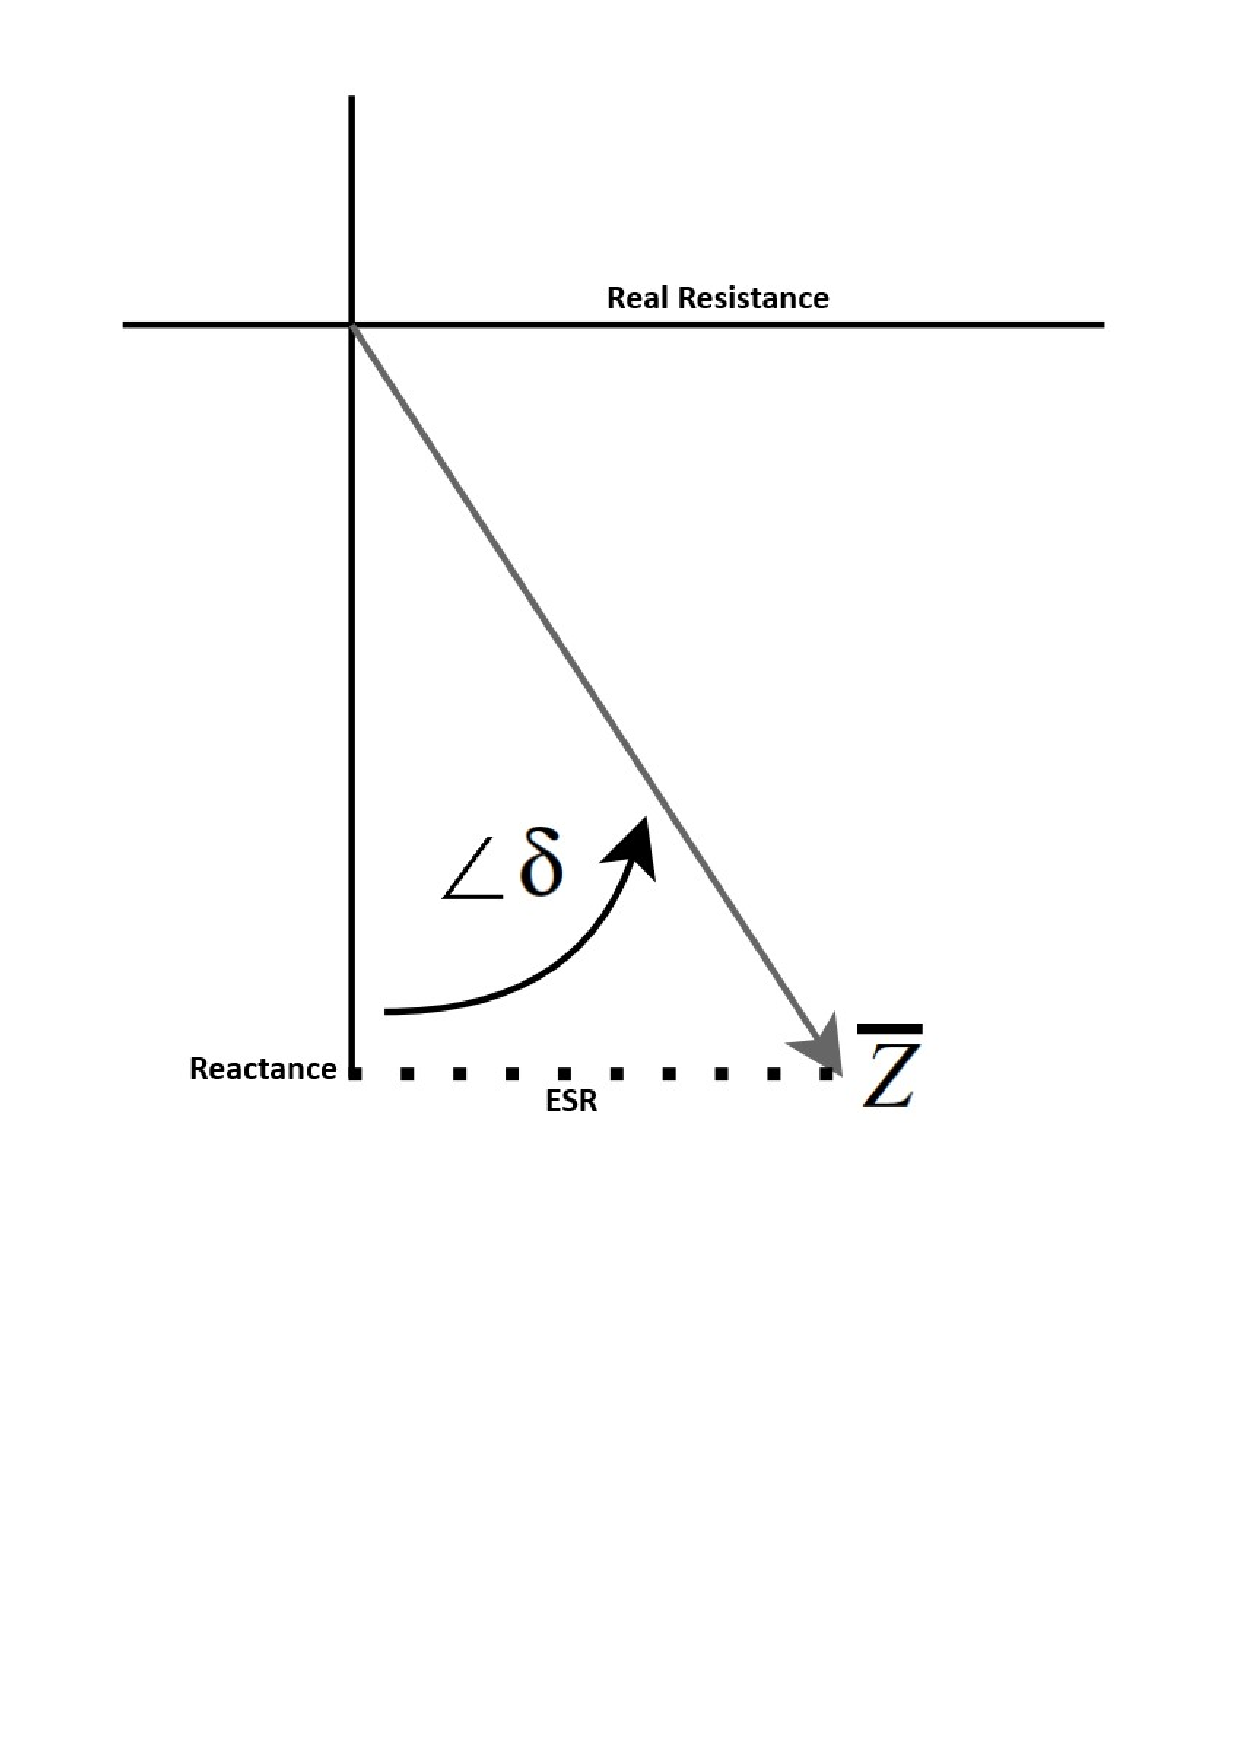
\includegraphics[clip, trim=0 275 0 0, width=0.4\textwidth]{Sections/4_TechnicalAnalysis/Figures/4_1_4_LossTangent2.pdf}
    \caption{The loss angle }
    \label{fig:4_1_1_LossTangent2}
\end{figure}

The loss angle on figure \refq{fig:4_1_1_LossTangent2} can be found in a number of ways, but it is often done with the tangent relation as shown in equation \refq{eq:4_1_1_LossAngle}. For this reason it is also called the \textit{loss tangent}.
\begin{equation}\label{eq:4_1_1_LossAngle}
    tan(\delta) =\frac{ESR}{|X|} 
\end{equation}
Where $X$ is the capacitive reactance in this case. The value $tan(\delta)$ is also called the \textit{dissipation factor} and $DF = tan(\delta)$. Electrolytic capacitors have relatively high ESR and will have a higher dissipation factor, so they will dissipate more power than a ceramic capacitor with a low dissipation factor would. The ESR can be found if the dissipation factor is known as shown in eq \refq{eq:4_1_1_ESR}.
\begin{equation}\label{eq:4_1_1_ESR}
    ESR =  tan(\delta)\cdot |X|
\end{equation}
An instrument measuring an impedance will, however, already know the ESR as the real part of the impedance.

Another common quantity that is also related to the loss tangent is the \textit{quality factor} which is simply the reciprocal of the dissipation factor as shown in eq \refq{eq:4_1_1_Q}.
\begin{equation}\label{eq:4_1_1_Q}
    Q = \frac{1}{DF} = \frac{|X|}{ESR}
\end{equation}
The quality factor will be high if ESR is low and vice versa.



